\section{Tables de plongée et ordinateur}

\begin{frame}{Tables MN90}
    \begin{columns}[c]
    \begin{column}{0.6\textwidth}
      \begin{itemize}
        \item Tables utilisées par la \textbf{FFESSM} : \textbf{MN90}.
        \item Objectif : éviter l'\textbf{accident de décompression}.
        \item Vitesse de remontée : entre \textbf{12 et 15 m/min}.
        \item Paliers à effectuer à la \textbf{profondeur} et pendant le \textbf{temps indiqués}.
      \end{itemize}
    \end{column}
    \begin{column}{0.4\textwidth}
      \centering
      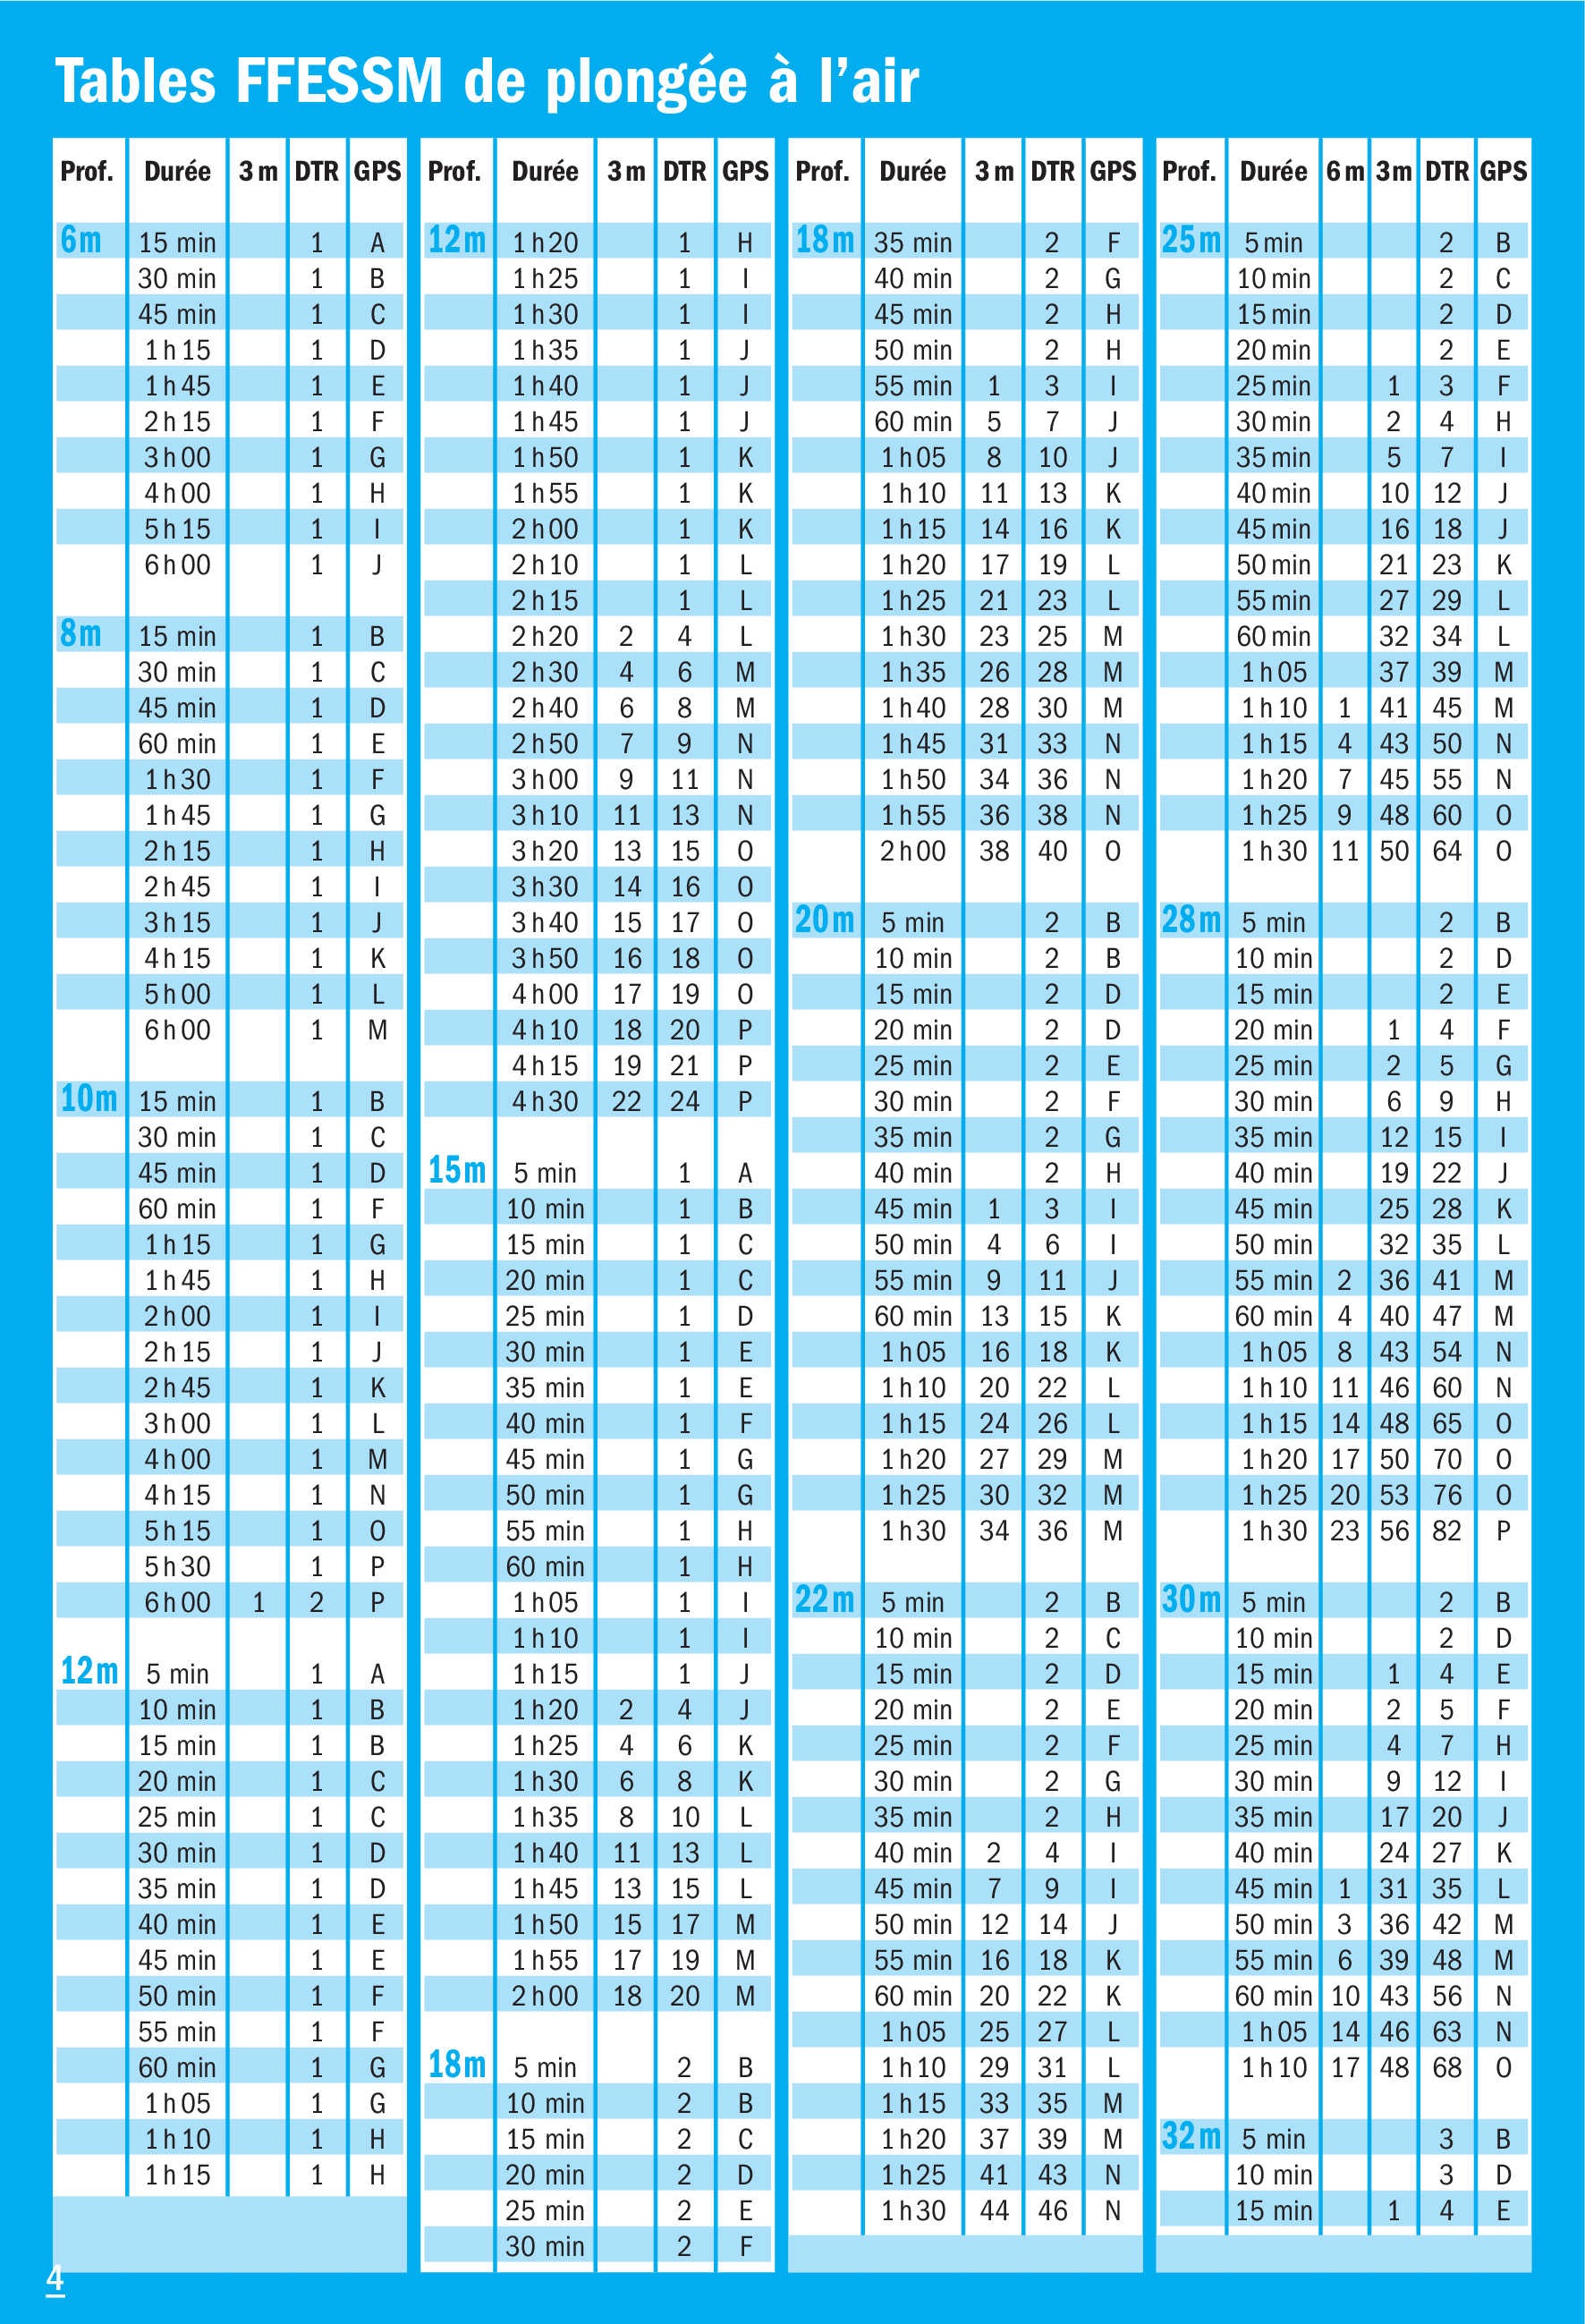
\includegraphics[width=0.79\textwidth]{images/mn90-exemple}
    \end{column}
  \end{columns}
\end{frame}

\begin{frame}{La Courbe de Sécurité}
  \begin{columns}[c]
    \column{0.5\textwidth}
    \textbf{C'est quoi ?}
    \begin{itemize}
      \item Pour chaque \textbf{profondeur}, elle indique le \textbf{temps maxi} de plongée
            possible \textbf{sans palier obligatoire}.
      \item Tant que l'on reste \textbf{sous} cette courbe, on peut remonter directement
            (en respectant la vitesse de remontée).
      \item Si on \textbf{dépasse} ces temps, des \textbf{paliers de décompression} deviennent
            nécessaires.
    \end{itemize}

    \column{0.5\textwidth}
    \centering
    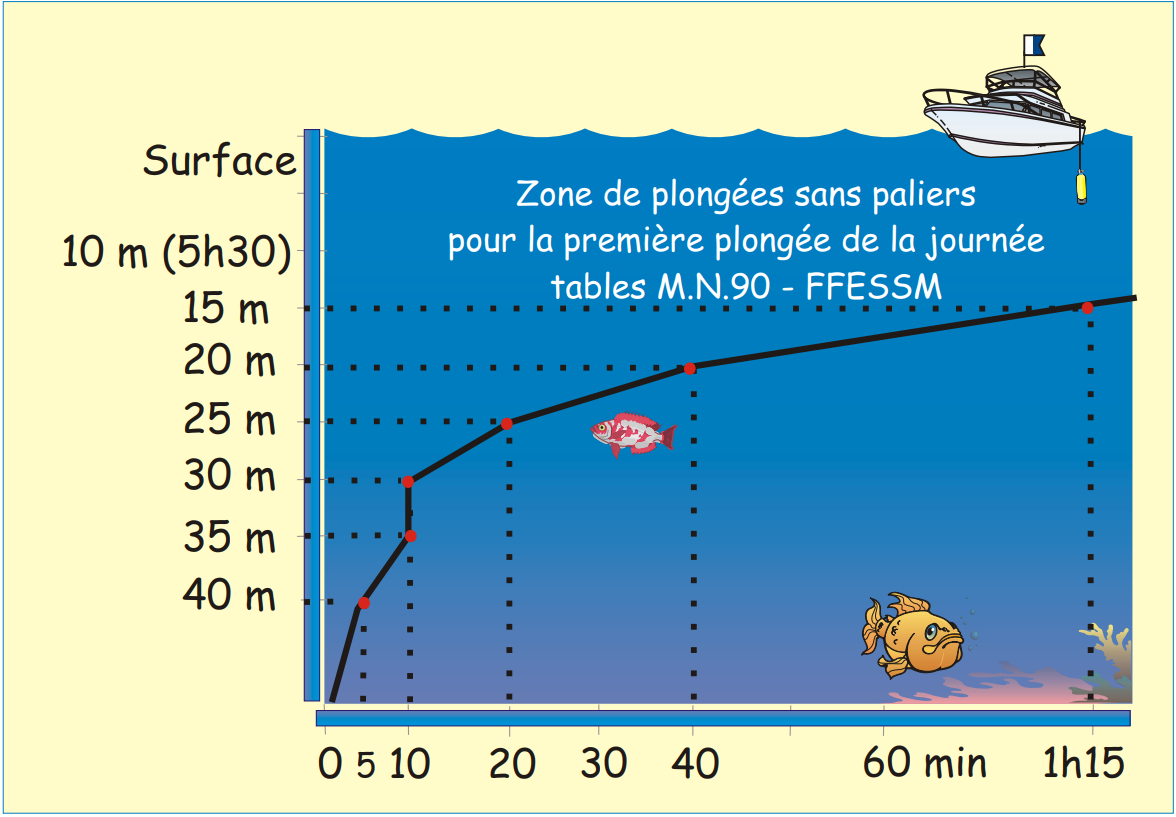
\includegraphics[height=0.6\textheight,keepaspectratio]{images/courbe-de-securite}
  \end{columns}
\end{frame}

\begin{frame}{Ordinateur de plongée}
  \begin{itemize}
    \item Principe identique aux tables mais calcul \textbf{en continu}.
    \item Capteur de pression $\Rightarrow$ profondeur instantanée.
    \item Calcule les \textbf{paliers} en fonction du profil réel.
    \item Indique la \textbf{vitesse de remontée} et les paliers à effectuer.
    \item Mémorise les paramètres pour les plongées suivantes.
  \end{itemize}
\end{frame}
